\documentclass[14pt]{extarticle}

\usepackage{fontspec}
\setmainfont{Times New Roman}

% размер полей
\usepackage{geometry}
\geometry{a4paper, top=2cm, bottom=2cm, right=1.5cm, left=3cm}

 %debugging
%\usepackage{showframe}

% полуторный интервал
\usepackage{setspace}
\onehalfspacing

% абзацный отступ
\setlength{\parindent}{1.25cm}

% выравнивание текста по ширине
\sloppy

% списки
\usepackage{calc} % арифметические операции с величинами
\usepackage{enumitem}
\setlist{
    nosep,
    leftmargin=0pt,
    itemindent=\parindent + \labelwidth - \labelsep,
}

% подписи к рисункам и таблицам
\usepackage{caption}
\renewcommand{\figurename}{Рисунок}
\renewcommand{\tablename}{Таблица}
\DeclareCaptionFormat{custom}
{
    \textit{#1#2#3}
}
\DeclareCaptionLabelSeparator{custom}{. }
\captionsetup{
    % хз какой это размер - 12 или нет, но выглядит меньше 14
    font=small,
    format=custom,
    labelsep=custom,
}

% картинки
\usepackage{graphicx}

% колонтитулы
\usepackage{fancyhdr}

% картинки и таблицы находятся именно в том месте текста где помещены (атрибут H)
\usepackage{float}

% таблицы
\usepackage{tabularray}

\graphicspath{ {2.2.2/models/} }
\begin{document}
\pagestyle{fancy}
\fancyhead{}
% disable header
\renewcommand{\headrulewidth}{0pt}
\fancyfoot[L]{Дубровских гр 221-361}
\fancyfoot[C]{ЛР 2.2.2}
\fancyfoot[R]{Продажа автотранспорта}
\singlespacing

\newpage
\begin{center}
    Министерство науки и высшего образования Российской Федерации
    Федеральное государственное автономное образовательное учреждение

    высшего образования

    \guillemotleft МОСКОВСКИЙ ПОЛИТЕХНИЧЕСКИЙ УНИВЕРСИТЕТ\guillemotright

    (МОСКОВСКИЙ ПОЛИТЕХ)
\end{center}
\noindent
\bigbreak
\bigbreak
\bigbreak
\bigbreak
\begin{center}
    ЛАБОРАТОРНАЯ РАБОТА 2.2.2

    По курсу Проектирования пользовательских интерфейсов в веб

    \textbf{Разработка карты путешествия клиента CJM (UJM, User Journey Map для веб-ресурса)}
    \bigbreak
    \bigbreak
    \bigbreak
    \bigbreak
    ТЕМА

    \guillemotleft\textbf{САЙТ ДЛЯ ПРОДАЖИ И ПОИСКА АВТОМОБИЛЕЙ}\guillemotright
\end{center}
\noindent
\bigbreak
\bigbreak
\bigbreak
\bigbreak
\bigbreak
\bigbreak
\bigbreak
\bigbreak
\bigbreak
\bigbreak
\hfill Выполнил

\hfill Дубровских Никита Евгеньевич

\hfill Группа 221-361
\bigbreak
\bigbreak
\bigbreak
\hfill Проверил

\hfill Натур ВВ
\vfill
\begin{center}
    Москва, 2024
\end{center}
\newpage
\onehalfspacing


\begin{center}
    \textbf{Лабораторная работа 2.2.2}

    \textbf{Разработка карты путешествия клиента CJM (UJM, User Journey Map для веб-ресурса)}
\end{center}

\textbf{Цель работы:} разработать карту путешествия пользователя CJM (User Journey Map для веб-ресурса)
\bigskip

\textbf{Задачи:}

\begin{enumerate}
    \item Построить карту путешествия пользователя User Journey Map для веб-ресурса
    \item Отметить этапы взаимодействия пользователя с интерфейсом веб-ресурса
    \item Прописать мысли, эмоции, страхи и ожидания пользователя на этапах использования веб-ресурса
    \item Обозначить возможные (спрогнозировать) критические точки и барьеры
    \item Предложить решение по устранению критических точек (барьеров) при проектировании интерфейса
\end{enumerate}
\bigskip

\textbf{Основные термины}

\begin{itemize}
    \item Customer Journey Map (CJM) - Карта путешествия клиента, визуальное представление пути пользователя при взаимодействии с сайтом или приложением.
    \item User Journey - Путь пользователя, описывающий его опыт взаимодействия с веб-ресурсом.
    \item Пользовательский опыт - Действия, чувства, страхи и мысли клиента во время взаимодействия с продуктом.
    \item Точки контакта - Моменты, когда пользователь взаимодействует с цифровым сервисом.
    \item Критические точки - Этапы, где пользователь испытывает негативные эмоции или сталкивается с барьерами.
    \item Барьер - Препятствие, мешающее пользователю достичь своей цели на сайте.
    \item Оптимизация - Процесс улучшения пользовательского опыта и устранения проблемных точек.
    \item USM (User Experience Management) - Управление пользовательским опытом.
    \item Этапы взаимодействия - Конкретные шаги, которые пользователь совершает на пути к своей цели.
    \item Мозговой штурм - Метод генерации идей для решения проблем и улучшения пользовательского опыта.
    \item Эмоции пользователя - Чувства, которые испытывает пользователь на разных этапах взаимодействия.
    \item Проблемные места - Участки на карте, где пользователи сталкиваются с трудностями или негативными эмоциями.
\end{itemize}
\bigskip

\textbf{Карта пользовательского опыта (UJM)}

\noindent
\begin{minipage}{\linewidth}
    \fbox{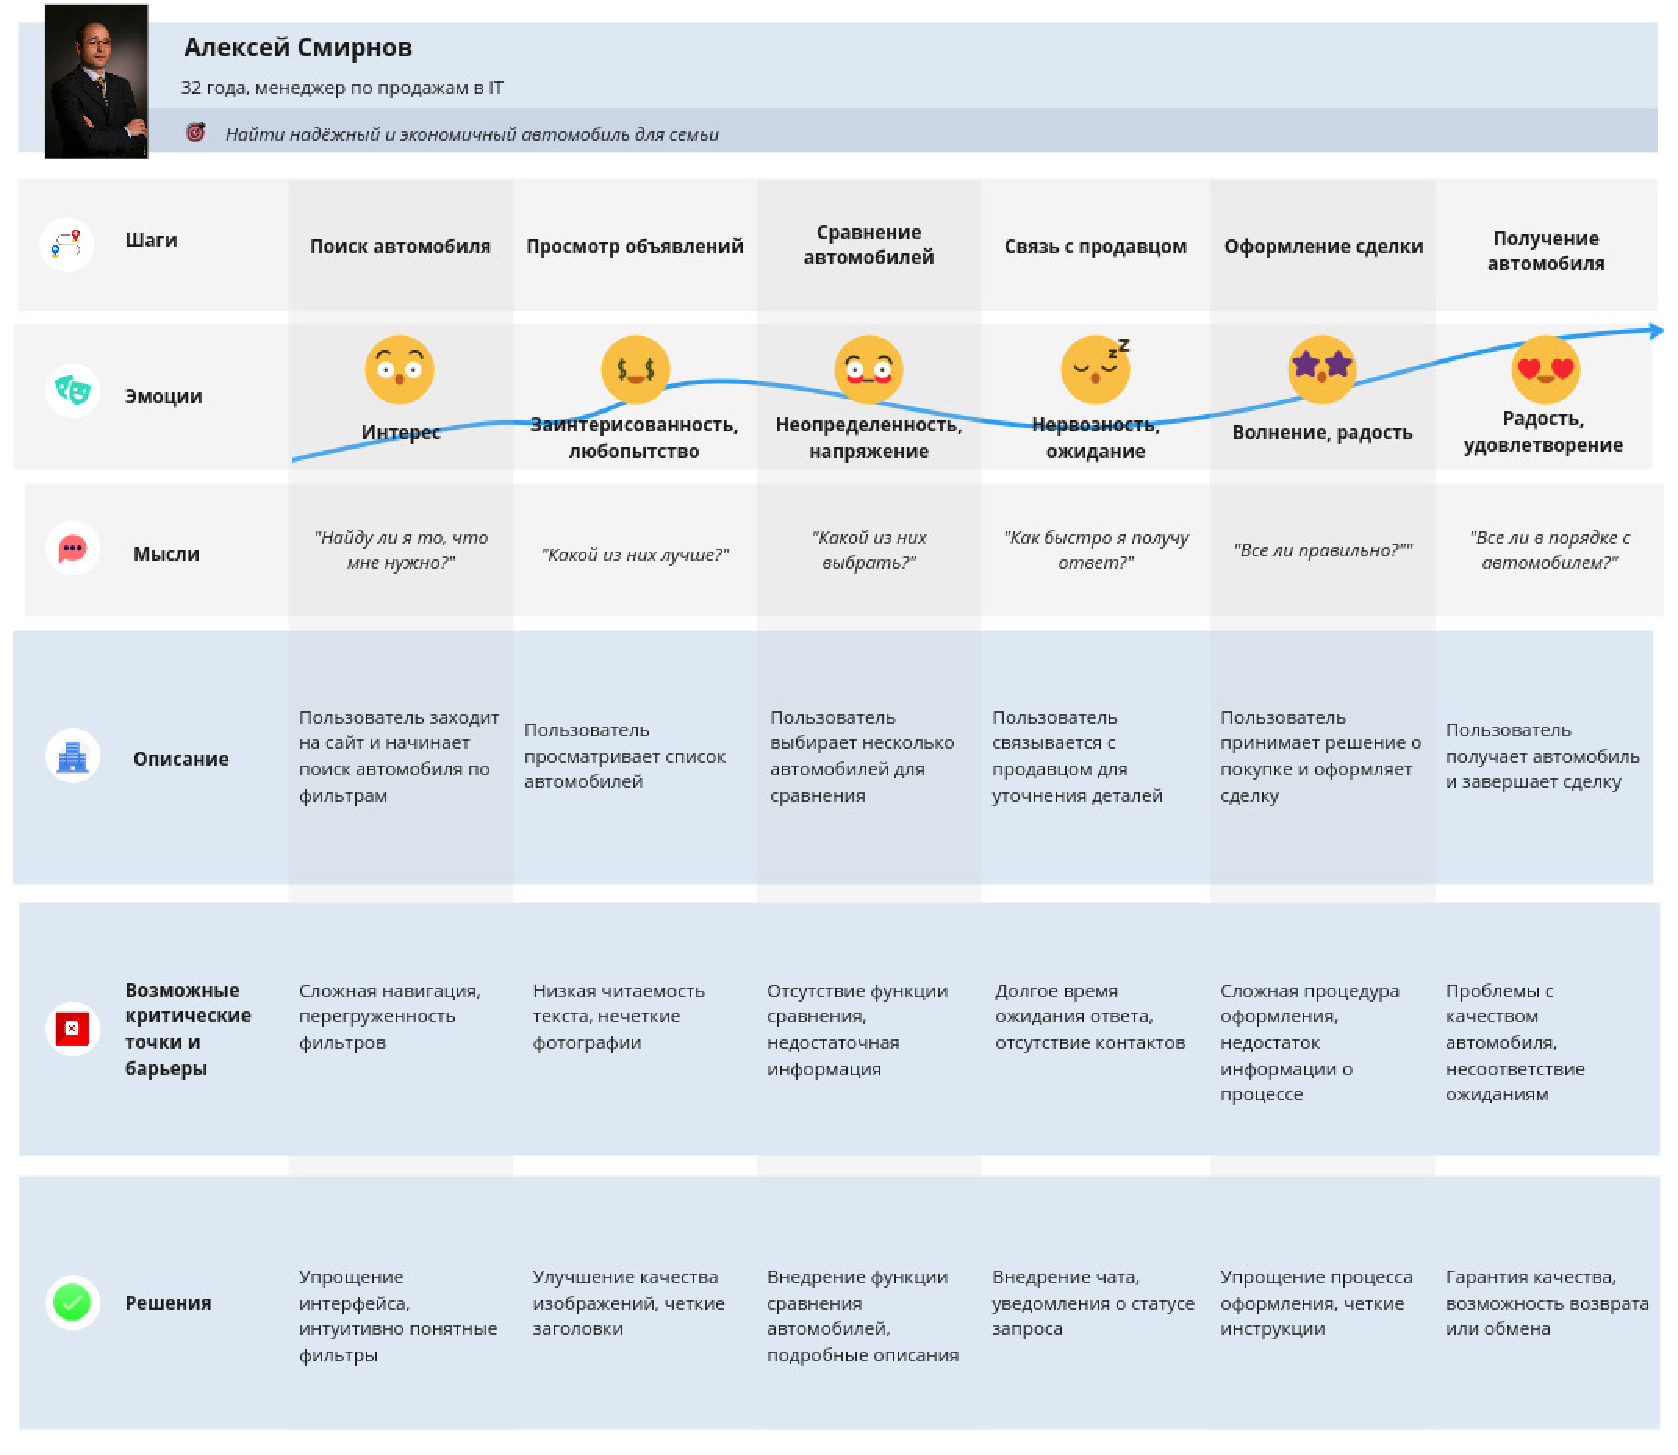
\includegraphics[width=\linewidth]{cjm}}
    \captionof{figure}{Карта путешествия пользователя}
\end{minipage}
\bigskip

\textbf{Контрольные вопросы и ответы}

\begin{enumerate}
    \item Что такое карта путешествия клиента Customer Journey Map (CJM)? Что такое User Journey Map?

Customer Journey Map (CJM) — это визуальное представление пути клиента при взаимодействии с продуктом или услугой, которое помогает понять его опыт и эмоции на каждом этапе.

        User Journey Map — это аналогичная концепция, но акцентируется на взаимодействии пользователя с веб-ресурсом или приложением.
    \item Как разрабатывается карта путешествия клиента User Journey Map?

Карта разрабатывается на основе сбора фактических данных о поведении пользователей, анализа их опыта, проведения исследований и веб-аналитики. Важно зафиксировать все этапы взаимодействия, эмоции и барьеры, с которыми сталкиваются пользователи.
    \item Где используется карта путешествия клиента User Journey Map?

Карта используется в различных областях, включая веб-дизайн, маркетинг, разработку продуктов и услуг, а также в UX/UI-дизайне для оптимизации пользовательского опыта и улучшения взаимодействия с клиентами.
    \item Какие задачи решает User Journey Map?

User Journey Map помогает:
        \begin{itemize}
            \item Понять психологию потребительского поведения.
            \item Проанализировать текущий опыт пользователя.
            \item Зафиксировать точки контакта с цифровым сервисом.
            \item Выяснить, что происходит с пользователем на каждом шаге его пути.
            \item Оптимизировать страницы сайта с учетом потребностей пользователей.
        \end{itemize}
    \item Какие барьеры могут возникать при использовании веб-ресурса (сайта или мобильного приложения)?

Возможные барьеры включают:
        \begin{itemize}
            \item Долгая загрузка страниц.
            \item Сложная навигация.
            \item Нечеткие заголовки и низкая читаемость текста.
            \item Ошибки на сайте (фактические, орфографические, технические).
            \item Обязательная регистрация для оформления заказа.
            \item Негативные отзывы о продукте или компании.
        \end{itemize}
\item Почему точки называются критическими? С какой целью их определяют и как устраняют?

Точки называются критическими, потому что в них пользователи испытывают максимальные негативные эмоции или сталкиваются с барьерами, мешающими им достичь своих целей. Их определяют для выявления слабых мест в пользовательском опыте. Устранение критических точек включает в себя анализ проблем, расстановку приоритетов, разработку плана действий и тестирование изменений для повышения удовлетворенности пользователей.
\end{enumerate}

\end{document}
